\documentclass{article}
\usepackage{graphicx}
\usepackage{standalone}
\usepackage{multicol}
\usepackage[parfill]{parskip}

% Used for sequence diagram
\usepackage{pgf-umlsd}
\usepackage{tikz}
\usetikzlibrary{shapes,arrows}

%used for subsubsubsections
\setcounter{tocdepth}{5}
\setcounter{secnumdepth}{5}

\usepackage{changepage}   % for the adjustwidth environment

% for currency
\usepackage{siunitx}

% syntax highlighting
\usepackage{listings} 
\usepackage{color}
\definecolor{lightgray}{rgb}{.9,.9,.9}
\definecolor{darkgray}{rgb}{.4,.4,.4}
\definecolor{purple}{rgb}{0.65, 0.12, 0.82}
\definecolor{codegreen}{rgb}{0,0.6,0}
\definecolor{codegray}{rgb}{0.5,0.5,0.5}
\definecolor{codepurple}{rgb}{0.58,0,0.82}
\definecolor{backcolour}{rgb}{0.95,0.95,0.92}
\lstdefinelanguage{JavaScript}{
  keywords={typeof, new, true, false, catch, function, return, null, catch, switch, var, if, in, while, do, else, case, break},
  keywordstyle=\color{blue}\bfseries,
  ndkeywords={class, export, boolean, throw, implements, import, this},
  ndkeywordstyle=\color{darkgray}\bfseries,
  identifierstyle=\color{black},
  sensitive=false,
  comment=[l]{//},
  morecomment=[s]{/*}{*/},
  commentstyle=\color{purple}\ttfamily,
  stringstyle=\color{red}\ttfamily,
  morestring=[b]',
  morestring=[b]"
}

\lstset{
   language=JavaScript,
   backgroundcolor=\color{lightgray},
   extendedchars=true,
   basicstyle=\footnotesize\ttfamily,
   showstringspaces=false,
   showspaces=false,
   numbers=left,
   numberstyle=\footnotesize,
   numbersep=9pt,
   tabsize=2,
   breaklines=true,
   showtabs=false,
   captionpos=b
}

% Hyperlinks
\usepackage[colorlinks,allcolors=blue]{hyperref}
\usepackage[normalem]{ulem}
\usepackage{xcolor}
\makeatletter
\begingroup
  \catcode`\$=6 %
  \catcode`\#=12 %
  \gdef\href@split$1#$2#$3\\$4{%
    \hyper@@link{$1}{$2}{\uline{$4}}% or \underline
    \endgroup
  }%
\endgroup

%Used for bibliography
\usepackage[british]{babel}
\usepackage[%
  autolang=other,
  backend=bibtex      % biber or bibtex
%,style=authoryear    % Alphabeticalsch
 ,style=numeric-comp  % numerical-compressed
 ,sorting=none        % no sorting
 ,sortcites=true      % some other example options ...
 ,block=none
 ,indexing=false
 ,citereset=none
 ,isbn=true
 ,url=true
 ,doi=true            % prints doi
 ,natbib=true         % if you need natbib functions
]{biblatex}
\addbibresource{../Bibliography/Bibliography}

\begin{document}
    \section{Project Analysis}
    \subsection{Overview}
	With this project I intended to create a proof-of-concept system for an `end-to-end' verifiable voting platform. While previous sections discussed the rationale, design and implementation, I now intend to analyse the projects success and viability.

	The project succeeds in presenting the protocol for an `end-to-end verifiable system' through use of Blockchain technology. The system is \textit{individually verifiable}, voters can check that their vote was successfully included in the Blockchain and can ensure that their vote was cast as intended (the stored result matches what the voter wanted). It is also \textit{universally verifiable} as anyone, whether they are participating in the election or not, can verify the results of the election \&, due to the systems design, be assured that each voter was only able to vote once per ballot.
	
	The associated costs with deploying a similar system on the scale of a general election look, not only feasible, but substantially less than current means. As this estimate is tied to the traded price of Ethereum we can expect some fluctuations in the actual cost but even with an exponential increase the costs should be less than a traditional election.
	
	Finally the scalability of the system, while not currently being able to process the vast number of transactions a general election would generate, does look like it will acquire the necessary throughput in the near future.
	
    \clearpage
    \subsection{Financial Feasibility}
	Using the Ethereum network as our distributed database comes at a cost. Obviously this requires computing power as the network ensures the integrity of the Blockchain along with processing new transactions into it and these computers need to be incentivized to continue providing this service.
	
	Is it important to understand what actually costs money in the system. You only pay for remote computation or data entry transactions so, in this system the only places we have an external cost are during poll creation and voting. Whenever we create a poll or a user votes we have to send Ether to the Ethereum network that collectively verifies your vote/poll and inserts it into the Blockchain. These are the two areas I have chosen to analyse and both cost money because we are writing data to the Blockchain.
	
	Each transaction has a fixed cost of gas which depends on several factors, such as the amount of computational steps it requires, this number cannot be adjusted as it depends on the transaction code being executed. Each transaction can also set a `gas limit' and a `gas price'. The `gas limit' is used to specify the upper bound of gas you are willing to pay for a transaction (unused gas is returned to the sender anyway) but is essentially used to ensure `buggy code' does not deplete your Ethereum account balance \citep{57_introduction_ethereum_frontier_guide_2017}. The gas cost of the transaction will be bought by the ether you have in your account at a price you specified with `gas price' Higher prices for each unit of gas means miners are more likely to run your contract or that you may overpay. 
	
	\subsubsection{Ballot Deployment}
	Creating a new ballot requires three things (as discussed in \hyperref[sec:CreatingANewBallotContract]{Creating A New Ballot Contract \ref*{sec:CreatingANewBallotContract}}) deploying the contract, adding the ballot options and finalizing the contract. More specifically, we are storing the following information into the Blockchain:
	\begin{itemize}
		\item \textbf{owner} - The address (20 bytes) of the ballot creator.
		\item \textbf{optionsFinalized} - Boolean value of whether the poll is set up.
		\item \textbf{ballotName} - Arbitrary length UTF-8 ballot name.
		\item \textbf{registeredVoterCount} - Integer count of registered voter addresses.
		\item \textbf{ballotEndTime} - Integer value of seconds since epoch.
		\item \textbf{votingOptions} - Dynamically sized array of the `VotingOption' structure (this structure contains a string name and integer vote count).
	\end{itemize}
	
	As you can see we do quite a lot in a varying number of transactions (varying because we add each option in a separate transaction and we can have an unlimited number of options). I calculated the costs associated with all of the ballots I publicly deployed over the course of my testing (\href{https://docs.google.com/spreadsheets/d/1dyLkpD-rdH4eHFEsdPrLEXX45YHl9XLGppbYgYYsTOo/edit?usp=sharing}{spreadsheet available here}) and found that while the average cost of fully deploying a contract (including adding multiple ballot options and finalizing) is around \pounds0.96 the individual cost vary considerably depending on the data being added (minimum cost was \pounds0.79 for a 2 option ballot and maximum was \pounds1.17 for a 6 option ballot). Changes in cost here seem to depend most on the number of options being added and the length of the string in each of those options.
	
\begin{figure}[h]
	\noindent  	
  	\makebox[\textwidth]{
  	    \begin{tabular}{ | l | S |}
    		\hline
    		\textbf{Description} & \textbf{Average Cost ({\pounds})}\\ \hline 		
			
			Average cost of the initial deployment. & 0.71 \\ \hline
			
			Average cost of adding a ballot option. & 0.05 \\ \hline
			
			Average cost of finalizing the contract & 0.02 \\ \hline
			
			Average cost to fully deploy a ballot & \\ (initial deployment, option addition and finalization). & 0.96 \\ \hline
    		   		
    		
    	\end{tabular}
  	}%
	\caption{Average cost of deployment actions (prices calculated April 2017).}
\end{figure}

	\subsubsection{Adding voters}
	The next cost incurred by the system is during the addition of voter addresses to the deployed ballot contract. Due to the fixed length of voter addresses (20 bytes) this type of transaction will always have the same amount of data being added to the blockchain; therefore we will always use the same amount of gas, 49100, for each transaction.

	\begin{figure}[h]
		\noindent
  		\makebox[\textwidth]{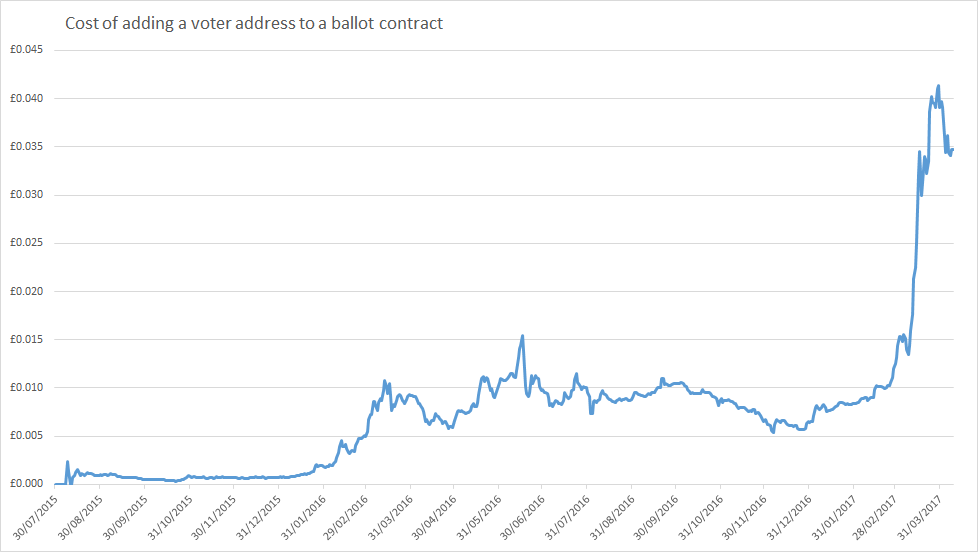
\includegraphics[width=1.07\textwidth]{cost_voter_addition}}%
		\vspace*{-0.3cm}
		\caption{Cost of registering a voter address over time tracking the inflation of Ethereum.}
	\end{figure}	
	\clearpage
	
	Therefore the only cost variable here is the `Gas Price' (the Ether price we buy a unit of gas for) which is tracked to the traded price of Ethereum. This means that the price we pay for adding a voter to a ballot contract will fluctuate over time with the price of Ethereum.

	Currently (April 2017) the price of Ethereum is around \pounds35.26 resulting in a price per address registered of \pounds0.04. Data released under the public information act \citep{69_statistics_from_2010_election} states that, during the 2010 UK General Election, there were 45,597,461 registered voters on the UK Parliamentary Register. To register this many people on our system at a cost of \pounds0.04 per voter, would equate to \pounds1,823,898. Even if we assume that the increased rate of inflation of Ethereum continues, an estimate of more than double the current Ethereum costs (\pounds £0.10 per voter) would cost around \pounds5 million. For perspective the cost to print, dispatch and return the postal votes for the 2010 election were around \pounds10.6 million \citep{70_what_price_democracy_counting_the_cost_of_uk_elections}.
	
	\subsubsection{Voting}
	The final area of cost relating the the ballot contracts is that of voting. And additional consideration here is allowing user to change their vote, as the cost incurred each time a vote is cast but more computation needs to be done on subsequent casts (due to the removal of the previous vote allocation).
	
	
	\begin{figure}[h]
	\noindent  	
  	\makebox[\textwidth]{
  	    \begin{tabular}{ | l | l |}
    		\hline
    		\textbf{Description} & \textbf{Average Cost ({\pounds})}\\ \hline 		
			
			Average cost of the initial vote. & 0.025 \\ \hline
			
			Average cost of re-voting. & 0.045 \\ \hline
    		   		
    	\end{tabular}
  	}%
	\caption{Average cost of per user voting and re-voting (prices calculated April 2017).}
	\end{figure}

	As you can see from the average costs table, the cost of re-voting is a little under half of the cost of the initial vote meaning it's not prohibitively expensive in relation to the original voting cost.
	
	If we calculate these prices with in relation to the registered number of voters in the 2010 election (45,597,461) \citep{69_statistics_from_2010_election} we find that cost for everyone to vote once would be around \pounds1,139,936.53 and the cost of everyone submitting a subsequent vote being \pounds2,051,885.75. 
	
	To represent this information in another form, these costs would mean (prices taken April 2017) that 1000 initial votes would cost the system \pounds25, 1000 re-votes would cost \pounds45, an individual casting their vote then changing their mind twice would cost \pounds0.115 and 1000 people doing so would cost \pounds115.

	\subsubsection{Cost Comparison}

	While initially looking at the above costs on a per-voter basis you might think that these prices are too high to be competitive with traditional voting techniques, however when broken down, we see a potentially different picture. As you might suspect, holding elections today is expensive and slow. The system is still based off of physical booths, paper ballots and requires humans to count the ballots (in some cases there are machines counting the ballots, but this is often more expensive than humans on a per voter cost basis \citep{71_arthur_2017}.)

	To compare this Ethereum-based voting system to the current voting system I'm using data from the 2010 UK General Election where the vote turnout was at 65.1\%. Therefore, out of 45,597,461 registered voters 29,991,471 actually voted \citep{72_voter_turnout_at_uk_general_elections}. The estimated the cost of this general election was \pounds113,255,271 \citep{70_what_price_democracy_counting_the_cost_of_uk_elections}  of which \pounds28,655,271 was the cost of distributing candidates mailings and a further \pounds84.6 million was for the conduct of the poll. This means that, on average, it cost about \pounds3.77 to register and count a vote but if we were to only take the costs for conducting the poll (\pounds84.6 million), it would cost \pounds2.82 to cast a single vote.

	Therefore we can compare the cost of using our Ethereum based voting system to the traditional system for this election. Remember that the average cost of the initial vote in our system was \pounds0.025, which means that if all of the voters were to use our system it would cost a total of \pounds749,786.75 to process these votes into the blockchain. Whilst this number might not be completely correct as we are presuming a lot (such as the price of Ethereum being the same, the fact that all of these votes would be using our system, and not counting the costs of running the backend of this system), it does put into perspective the potential cost savings when compared to traditional means.
	
	To compare, the traditional voting system would be around 3800\% (38x) more expensive than a blockchain voting system in this scenario. This breaks down to the cost of casting each vote being \pounds2.82 in the traditional system to \pounds0.025 in our system.
	
	With this margin of cost savings we could afford to let every voter re-vote up to 21 times and still cost less that the traditional system. This is likely an underestimate of the actual number as its unlikely everyone would choose to re-vote.
	
	\clearpage
	\subsubsection{Cost minimization strategy}
	In Ethereum, each instruction in the Turing complete scripting language has an associated cost when executed, along with additional costs for writes to the Blockchain. These costs are counted in gas and the user specifies the price per gas unit that they are willing to pay. Permanent storage to the Blockchain dominate transaction costs, it currently costs 3 gas to perform an addition but 20,000 gas to store a single 256-bit integer.
	
	As each operation consumes a calculable amount of gas we can aim to minimize the gas used through careful contract design. Simplifying the contract as much as possible is a good way to start but we could also look into more subtle ways to reduce costs such as choosing storing the voters ballot choice as an index (integer) rather than a string.
	
	We can also look at the contract at a higher level, for example the contract I have written for this system uses multiple transactions to setup the contract (one for the initial deployment, one for each ballot option and a one to finalize). I was unable (at the time of writing the contract but future language updates should fix this) to send an arbitrary number of strings in the constructor of the contract due to current limitations of the EVM. Therefore I settled on using multiple transactions to maintain this functionality rather than compromise the contracts usability. Once the EVM has been updated and is able to handle this sort of information, we could compress this into one singular call to deploy the contract with all of the ballot options minimizing the cost of setting up a ballot.
	
	There is also the potential for analysis of the optimal gas price to set for each transaction. As miners can choose which transactions to accept based on the amount of computation and the gas price of the transaction, we could work out the most effective price to use at a given moment in time to minimize both the cost to us and the transaction confirmation time. Though the savings per transaction would likely be minimal, when scaled to the numbers involved in a general election the compounded savings could be of reasonable note.
	
		
	\clearpage
	\subsection{Scalability}
	Throughout this paper I have been working on the assumption that the Ethereum network would be able to handle the amount of transaction volume a general election would bring. 
	
	At the current gas limit of 4,019,884, at the cost of 42182 gas per initial vote, we could only register some 95 votes every 12 seconds. That is about 684,000 in a day. Therefore, holding the General Elections on the Ethereum Blockchain would take around 43 days to complete. This is of course not acceptable and therefore can say that, at the current time, the Ethereum Network does not have the capacity to scale to this level. This problem is more general than the Ethereum network and is currently inherent to blockchain technologies, the same scalability problems currently exist across all other protocols.
	
	However, Ethereum has some scaling properties already built in. While there is a `Block Gas Limit' governing how many transactions can be confirmed in a single block, this limit (unlike other protocols such as Bitcoin) is not fixed and does in fact have the ability to adjust after every confirmed transaction. Miners can choose to change the gas limit $\pm\frac{1}{1024}$ depending on the networks gas consumption at a given time. Block gas limits scale indefinitely \citep{73_wood_2017} so under excessive demand we can expect to see more transactions per block.
	
	A more recent and promising development was that Vitalik Buterin, founder of Ethereum, has laid out an ambitious roadmap with ``unlimited'' transaction scalability within two years \citep{74_ethereum_announces_unlimited_scalability_roadmap}. The changes have been outlines in a yellow-paper \citep{73_wood_2017} and introduce the idea of `sharding' to the Ethereum network which would ultimately mean that not every node needs to process every transaction. 
	
	\textit{``The long term goal for Ethereum 2.0 and 3.0 is for the protocol to quite literally be able to maintain a blockchain capable of processing VISA-scale transaction levels, or even several orders of magnitude higher, using a network consisting of nothing but a sufficiently large set of users running nodes on consumer laptops.''} - Vitalik Buterin, 2016 \citep{74_ethereum_announces_unlimited_scalability_roadmap}.
	
	The changes outlined in this paper would allow throughputs of around 10000+ tx/sec \citep{75_eip_105} which would more than cover the needs of our system. Currently, Ethereum is the only protocol who is actively working towards sharding as a solution to the scalability problems which gives further validity to the choice of using it for this system.
	
	\clearpage
	\subsection{Privacy}
	Voter privacy (i.e. the inability to link a voter to a vote) is the most important property of a voting system because once it is compromised, coercion and collusion cannot be avoided and therefore no other requirement can be assured \citep{48_safevote_2001}. 
	
	The design of the system ensures that, with the exception of the securely stored private key of each voter, there is no information retained which could link a user account (and the individual behind it) to an Ethereum address. Unfortunately, there is still a degree of trust which must be instilled in the central authority that they are running this system as described and maintaining this secrecy which many users may be unwilling to do. While open sourcing the codebase could alleviate some this there will always be some parts of the system behind closed doors though how to gain the public's trust in such a system is beyond the scope of this paper.
	
	\subsubsection{Voter Obfuscation}
	Due to the public nature of the votes being cast in a Blockchain, we need to be aware of the possibility for a voter to inadvertently leave a trail which could be followed and directly identify them. The main concerns here would be based around some form of statistical analysis being able to discern potentially identifying traits of a voters Ethereum address. 
	
	\paragraph{New voting address per ballot}
	\hfill \break \break
	One possible way for an address to become less anonymized would be if it was used for multiple ballots. For example, if you could see that an address voted in a particular regional ballot and that they were the only ones to vote for a particular candidate while being externally vocal about their opinions on this particular ballot. You could determine who that individual was and then, because they used the same address for other ballots, see other voting choices.
	
	The system actually takes steps to eliminate this possibility. We generate a new, unique voting address for each ballot the voter registered to participate in. As address creation is very cheap and the address space is incredibly large, it makes sense to generate a new address each time while incurring almost no additional overhead. This means that there is no chance to link addresses across ballots, as each address is only used for a single ballot.
	
	\clearpage
	\paragraph{Transaction timings}
	\hfill \break \break
	Another possibility for statistical analysis could be found in the timing of transactions being submitted. For example while testing the system, as there was very few users actively voting concurrently, it was easy to determine which transactions were mine as they were the only ones being sent. Applying this more generally, maybe an ISP could see the times you accessed the voting web interface and if there were sufficiently few transactions during that time we could trivially link your voting choice to you.
	
	While this problem is significantly reduced when the system is used by a larger number of people, we could also employ tactics such as modulating the `gas price' of the transaction to increase the amount of time between it being submitted and confirmed. Whilst its desirable to be able to see your vote as `confirmed' almost instantly, it is not strictly necessary. As long as you can see that is has been included in the pool of unconfirmed transactions you can assume with relative certainty that is will be accepted at some point in the future.
    
    \subsubsection{Voter coercion}
    Though illegal the removal the guaranteed secrecy of a polling booth does open the possibility for increased levels of voter coercion when using this system.    
    
	\paragraph{Vote buying}
	\hfill \break \break
	The transparency of this system undermines the basis of vote buying. To ensure that the purchased votes were not merely promised, the vote buyer would be compelled to collect vote receipts and to record the identities of the sellers. He would also have to ask the vote seller to forgo payment until after the election results had been finalized (as a voter can change their vote up to the election deadline). Therefore as the sellers would have no means of enforcing the completion of the transaction the low level of trust between buyer and seller would make this form of vote buying unlikely.

	Even if a valid voting receipt, in the form of a transaction hash, was presented for payment after the election it would similarly be of no value. Since all votes are publicly broadcast, anyone could submit any transaction hash that was cast in favour of a particular candidate as this receipt is proof that a ballot has been cast, but gives no indication who cast it, a buyer is unlikely to pay in this scenario.

	\clearpage
	\paragraph{Forced voting}
	\hfill \break \break
	One concern unique to this way of voting, is the guaranteed return of a receipt for each vote cast in the form of the transaction hash. The returning of this hash is inescapable, as its a core part of the blockchain functionality and provides the only way for a voter to validate that their transaction was included into the blockchain. 
	
	The problems of community pressure, are mitigated by the fact that (as mentioned in the previous section), a voter can provide any transaction hash as a receipt and it is not individually identifiable. Therefore requesting a receipt to prove the way an individual voted does not work.
	
	A more realistic problem however is, due to the lack of a polling booth, individuals can be forcibly made to vote in a particular way. I was unable to think of a direct way to combat this, however I propose a method for a voter to discreetly mark these forced ballots as such and for them to not be counted in the ballot tally.
	
	As the user is required to enter a password to unlock the Ethereum account before a transaction can be authorized, I would introduce the idea of a `panic password' at this stage. Panic passwords gained traction as a safety measure for ATM transactions. It is a special password or set of actions which the user can trigger to alert the server that the user is under duress. In this system it could be that the user enters their password in reverse to trigger the panic status.
	
	Once this occurs, the system continues as usual processing the transaction and providing a receipt except with the addition of a flag as part of the transaction which ultimately invalidates this vote in the contract. This would mean the person forcing the vote would be none the wiser as externally it would appear the same as a regular vote.	
	
	\clearpage
	\subsection{System security}
	\subsubsection{The Ethereum Network}
	 With the scope of this project aiming to design a secure voting system, possibly usable in a general election, it's essential to confirm the level of security and to understand the risks involved with the Etherum network.

Ethereum while not branded as a cryptocurrency, is often traded on cryptocurrency exchanges and as the name suggests, cryptography is a central part of the protocol. Ethereum makes use of the KECCAK-256 cryptographic hashing function (essentially SHA-3 before standardization).

Signatures in Ethereum are performed exactly the same as in conventional public-key cryptography. We can verify that Alice is the owner of a transaction because she has signed it with her private key, which can then be verified with her public key. Ethereum uses the ECDSA elliptic curve for generating the key pairs which appears to have been chosen for possible speed optimizations in the future \citep{41_yang_2011}. Attacks here could involve breaking the underlying elliptic curve cryptography either by solving the discrete logarithm problem (which could be possible with quantum computers, but there is currently no efficient non-quantum algorithm), or by finding vulnerabilities in the specific curve chosen.

As with most public-key cryptography, Ethereum does not sign the entirety of the transaction as this would be too expensive. Instead, it signs a hash which can then be checked against the transaction to verify its integrity. If we could break the hash function, it could be possible to generate a secondary input transaction to hash to the same value as an original. This could then be used to perform a signature replay attack to forge a transaction.

The likelihood of either of these two scenarios being immediate threats is however, relatively low. Ethereum uses industry standard technology and a breach in any of the underlying cryptography would undermine a large proportion of the security we enjoy on the internet. 

Despite the underlying cryptography being secure, there are still a number of possible attacks which could be utilised against the network. While a dishonest miner cannot generate Ether (illegitimately), steal Ether from an account or make payments on your behalf (pretend to be you), they could delay or refuse the relaying of valid transactions to other nodes, attempt to create blocks which exclude specific transactions of their choosing or attempt to create a longer blockchain that would render previously accepted blocks invalid \citep{22_brave_new_coin_2016}. However all of the above require the attacker to have sufficient block creation power, effectively a 51\% attack on the network. When an individual or group owns more than half of the network they could produce enough ``computational work'' to convince others that their blockchain is the best choice \citep{41_yang_2011}.

This became a real threat on the Bitcoin network in January of 2014 as the mining group \textit{Gash.io} started to approach 50\% of the mining power of the entire network. At one point the group had collectively solved 42\% of the blocks in a 24 hour period \citep{42_liu_2014}. The situation was resolved without incident, due to miners leaving \textit{Gash.io} for smaller pools, as well as the pool’s own decision to stop accepting new miners \citep{41_yang_2011}.
	
	\subsubsection{Voter key management}
	As with the various types of Bitcoin and Ethereum wallet software available there is always a trade-off between user managing their own keys and online services doing it for them. Storing private keys on behalf of users is a very dangerous thing to do, especially if we are talking about a general election which would be of great interest to hackers. However, the truth of the matter is that the vast majority of people lack the skills needed to properly protect such information by themselves.
	
	For this reason the system should be designed to securely store the encrypted private keys of each user in its internal database. This encryption should be of sufficient strength, AES-256, and while being password based we should enforce a different password than the one a voter uses to log into the system (as this could present a risk that if the server becomes compromised an attacker would trivially be able to affect the votes in the blockchain).

	This is a difficult problem to solve, companies such as LastPass get around this by only ever seeing an encrypted version of your private data (as encryption and decryption happen client side). This approach opens the user to the possibility of being compromised and also would also require sending the private key over the wire to authenticate a transaction (though this concern may be mitigated with secured connections).
		
	A potential alternative could be to enforce the user to print out their private key (similarly to a paper wallet) in the form of a QR code. This could then be scanned in when necessary to unlock the account and authorize a transaction. Although this approach might reduce the chances of keys on a voters computer being compromised, it still places the security of the voters ballot in the voters hands.

	\subsubsection{Loss of Ether}
	\label{sub:LossOfEther}
	Because we fund each users account with enough Ether to submit a transaction vote, there is potential for a large scale loss of Ether either to occur. This could be through over supplying ether to accounts or by users attempting to game the system. 
	
	For the proof-of-concept, the system currently supplied 0.005 Ether to each registered account so that they may perform around 4 to 5 transactions. This is obviously not the best way to implement this when scaling to the level of a general election as, say for example the user only votes once then the remaining Ether goes unspent at cost to the system. It also incentives people to attempt to game the system as they see this as free money (albeit a very small denomination) which they may attempt to transfer into a private account.
	
	As a potential future improvement I suggest a system where we always fund the voter address with enough Ether to conduct one additional vote. This amount should be calculated based on predicted gas and Ether prices and should include a degree of leniency in favour of over funding. When a user submits a vote, their account is automatically topped up the to required level to be able to submit another one. In this way, we eliminate the over funding problem for those accounts who were never going to re-cast their votes while still allowing those who do wish to, unlimited voting opportunity.
	
	This system however could be easily exploited due to the slight over funding to compensate for price fluctuations. A user could re-vote multiple times to accumulate an excess of Ether which could then be siphoned off. To compensate for this, some form or rate-limiting could be employed (maybe 3 re-votes per hour) along with a check of whether the voters account has enough to cast another vote before funding it again.
	
	\subsubsection{Individual computer security}
	Moving an election of any type away from the security of a polling booth and on to individuals computers, phones and laptops presents many security issues. The potential for an attacker to compromise an uneducated user's computer is relatively high and an event such as a general election would undoubtedly produce more attempts to do so.	As voting options are conducted through a web interface, the possibility of XSS attacks or attempts to miss-represent one voting option as another must be considered.
	
	Therefore alongside strong secure design, as a minimum voters should be educated on basic computer security that would allow them to increase the difficulty for an attacker to compromise an individual voter.	
	
	We could also enforce certain security requirements on the user, such as running an up-to-date OS version or requiring certain security software to be installed and active. But this must not raise the barrier to entry so much that we alienate a group of the voting populous (for example the elderly might not be able to easily conform to these requirements).
	
	\clearpage
	\subsubsection{Direct contract interaction}
	For the most security conscious we could allow direct contract interaction from an individual. This would likely only be undertaken by a handful of people but it would still require them to use some parts of the system to submit an address which they wish to use and have it added to the ballot contract in the blockchain. Ultimately though this would still be heavily reliant on system interaction which would be what people wishing to conduct this interaction will be most critical of.
	
	It may be possible to move more of the inner workings of the system on to the blockchain its self. Although some form of verification will still need to happen, users could interact with a smart contract in order to have their private addresses added to the list of allowed voters. Having more of the system become transparent would be beneficial not only to these more sceptical individuals but increase trust in the system as a whole.
    
\clearpage
\subsection{Improvements}
Reflecting upon the project, there are a number of design decisions which I would consider doing differently next time.

\subsubsection{Implementation}
Firstly, I would run Geth (the Ethereum software) in its own Docker container. Currently it is being run inside the ``Online Ballot Regulator'' and could be easily extracted for a more modular system. Running it in its own container would further segregate the various sections of the application providing increased security and decouple the files of the ``Ballot Regulator'' from any files generated by Geth.

I would also serve the web application over Apache (or a similarly established software). Currently the system is running off of Django's built in webserver which, while fine for development, it is a stripped-down, very basic, single-threaded server for the purposes of development and has not gone through the required security audits or performance tests for production deployment. Transferring the server over to Apache would be trivial to setup with the WSGI interface.

\subsubsection{Protocol}
There is a glaring omission in the design of the ballot contract, the opportunity for voters to practice their right to suffrage. Currently the ballot contract template does not add any option for a `non-vote' which should be included to maintain voter rights.

This could be easily implemented with minimal change to the solidity contract. We could add an extra ballot option titled `non-vote' or similar during the finalization state of ballot creation meaning it would be automatically applied to all ballots.

I would also re-implement the way voter accounts receive funding to allow them to vote (also discussed in the \hyperref[sub:LossOfEther]{Loss of Ether \ref*{sub:LossOfEther}} section). Essentially I would change it to a top-up system where more Ether is allocated to your account when you vote rather than giving it all to you in one go. This reduces unnecessary allocation of funds to voters who will only use their initial vote and reduces the likelihood of an individual attempting to game the system.


\end{document}
